\documentclass[landscape]{article}
\usepackage{tikz}
\usepackage[default]{sourcesanspro}
\usepackage[T1]{fontenc}

\pagenumbering{gobble}

\newenvironment{sentencediagram}[3]
    {
        \begin{center}
            {
                \fontfamily{cmr}\selectfont
                #1 \newline
            }

            \footnotesize #2, \textit{#3}
            \LARGE 
    }
    {\end{center}}

\definecolor{subjectnoun}{RGB}{106,120,132}
\definecolor{copula}{RGB}{124,139,111}
\definecolor{subjectcomplement}{RGB}{77,47,13}
\definecolor{conjunction}{RGB}{56,84,129}
\definecolor{preposition}{RGB}{32,129,159}
\definecolor{directobject}{RGB}{231,51,143}

\begin{document}

\begin{sentencediagram}{It was a bright cold day in April, and the clocks were striking thirteen.}{George Orwell}{1984}
    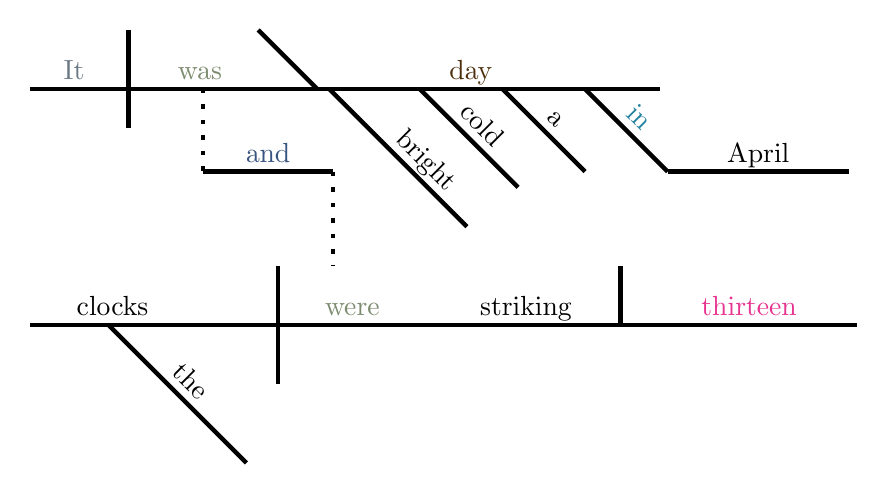
\begin{tikzpicture}
        \tikzstyle{every node} = [above=-0.15cm]
        \draw[ultra thick] (-5, 1.75) -- (3, 1.75)
            node[pos=.07, text=subjectnoun]{\strut It}
            node[pos=.27, text=copula]{\strut was}
            node[pos=.7, text=subjectcomplement]{\strut day};
        \draw[ultra thick] (-3.75, 2.5) -- (-3.75, 1.25);
        \draw[ultra thick] (-2.1, 2.5) -- (-1.35, 1.75);
        \draw[ultra thick] (-1.2, 1.75) -- (-0.3, 0.85)  -- (0.55, 0)
            node[sloped, pos=0.2]{\strut bright};
        \draw[ultra thick] (-0.05, 1.75) -- (1.2, 0.5)
            node[sloped, pos=0.5]{\strut cold};
        \draw[ultra thick] (1, 1.75) -- (2.05, 0.7)
            node[sloped, pos=0.5]{\strut a};
        \draw[ultra thick] (2.05, 1.75) -- (3.1, 0.7)
            node[sloped, pos=0.5, text=preposition]{\strut in};

        \draw[loosely dotted, ultra thick] (-2.8, 1.75) -- (-2.8, 0.7);
        \draw[ultra thick] (-2.8, 0.7) -- (-1.15, 0.7)
            node[pos=.5, text=conjunction]{\strut and};
        \draw[ultra thick] (3.1, 0.7) -- (5.4, 0.7)
            node[pos=.5]{\strut April};
        \draw[loosely dotted, ultra thick] (-1.15, 0.7) -- (-1.15, -0.5);

        \draw[ultra thick] (-5, -1.25) -- (5.5, -1.25)
            node[pos=.1]{\strut clocks}
            node[pos=.39, text=copula]{\strut were}
            node[pos=.6]{\strut striking}
            node[pos=.87, text=directobject]{\strut thirteen};
        \draw[ultra thick] (-1.85, -0.5) -- (-1.85, -2.0);
        \draw[ultra thick] (2.5, -1.25) -- (2.5, -0.5);
        \draw[ultra thick] (-4, -1.25) -- (-2.25, -3.0)
            node[sloped, pos=.5]{\strut the};
    \end{tikzpicture}
\end{sentencediagram}

\end{document}
